\documentclass{article}\usepackage[]{graphicx}\usepackage[]{color}
%% maxwidth is the original width if it is less than linewidth
%% otherwise use linewidth (to make sure the graphics do not exceed the margin)
\makeatletter
\def\maxwidth{ %
  \ifdim\Gin@nat@width>\linewidth
    \linewidth
  \else
    \Gin@nat@width
  \fi
}
\makeatother

\definecolor{fgcolor}{rgb}{0.345, 0.345, 0.345}
\newcommand{\hlnum}[1]{\textcolor[rgb]{0.686,0.059,0.569}{#1}}%
\newcommand{\hlstr}[1]{\textcolor[rgb]{0.192,0.494,0.8}{#1}}%
\newcommand{\hlcom}[1]{\textcolor[rgb]{0.678,0.584,0.686}{\textit{#1}}}%
\newcommand{\hlopt}[1]{\textcolor[rgb]{0,0,0}{#1}}%
\newcommand{\hlstd}[1]{\textcolor[rgb]{0.345,0.345,0.345}{#1}}%
\newcommand{\hlkwa}[1]{\textcolor[rgb]{0.161,0.373,0.58}{\textbf{#1}}}%
\newcommand{\hlkwb}[1]{\textcolor[rgb]{0.69,0.353,0.396}{#1}}%
\newcommand{\hlkwc}[1]{\textcolor[rgb]{0.333,0.667,0.333}{#1}}%
\newcommand{\hlkwd}[1]{\textcolor[rgb]{0.737,0.353,0.396}{\textbf{#1}}}%

\usepackage{framed}
\makeatletter
\newenvironment{kframe}{%
 \def\at@end@of@kframe{}%
 \ifinner\ifhmode%
  \def\at@end@of@kframe{\end{minipage}}%
  \begin{minipage}{\columnwidth}%
 \fi\fi%
 \def\FrameCommand##1{\hskip\@totalleftmargin \hskip-\fboxsep
 \colorbox{shadecolor}{##1}\hskip-\fboxsep
     % There is no \\@totalrightmargin, so:
     \hskip-\linewidth \hskip-\@totalleftmargin \hskip\columnwidth}%
 \MakeFramed {\advance\hsize-\width
   \@totalleftmargin\z@ \linewidth\hsize
   \@setminipage}}%
 {\par\unskip\endMakeFramed%
 \at@end@of@kframe}
\makeatother

\definecolor{shadecolor}{rgb}{.97, .97, .97}
\definecolor{messagecolor}{rgb}{0, 0, 0}
\definecolor{warningcolor}{rgb}{1, 0, 1}
\definecolor{errorcolor}{rgb}{1, 0, 0}
\newenvironment{knitrout}{}{} % an empty environment to be redefined in TeX

\usepackage{alltt}

\usepackage{multicol}
\usepackage{geometry}
\usepackage{amsmath}

\geometry{
 a4paper,
 total={210mm,297mm},
 left=20mm,
 right=20mm,
 top=20mm,
 bottom=20mm,
 }
\IfFileExists{upquote.sty}{\usepackage{upquote}}{}
\begin{document}

\title{GTEx expression data\\-\\
        Rainet project}
\author{Diogo Ribeiro, Lionel Spinelli, Andreas Zanzoni, Christine Brun}
\maketitle

\section{Introduction} 

We plan to use the GTEx V6 dataset (http://gtexportal.org), Human genome-wide RNA-seq expression data, to add RNA expression information in our RAINET database. 
The purpose is to use the expression to filter out Protein-RNA interactions that unlikely to occur in vivo. We will apply a threshold of expression value to ascertain the potential presence of each protein and RNA in a certain tissue, and excluded interactions where one or both of the interaction partners are missing. 
We will extrapolate the protein presence or absence by the expression of their respective mRNA. It as been shown (REF) that prediction of protein presence is accurate when its RNA is expressed above ..X.. rpkm. \par
The GTEx dataset contains full RNA-seq experiments done on hundreds of individuals, and retrieved from several physical locations / tissues. 
The GTEx project provides downloadable data where the reads have been mapped to human genome and rpkm values were calculated for each GENCODE (v19) transcript (note that this includes all types of RNAs: mRNAs, lncRNAs, snoRNAs, etc).
They provide several files, among them the description of the individual RNA-seq samples, including the tissue and body site:
GTEx\_Data\_V6\_Annotations\_SampleAttributesDS.txt. \par
The file with the rpkm values contains values for each transcript for each sample:
GTEx\_Analysis\_v6\_RNA-seq\_Flux1.6\_transcript\_rpkm.txt. \par
For insertion of expression data into our RAINET database we want to transform the GTEx data to have a single expression value for each RNA-tissue pair, therefore, exclude the sample/individual dimension from the data. 
We will first perform a rough analysis of expression values distributions across samples to reach the best solution for transforming this data.

\section{Samples variability per tissue}

Number of samples per tissue using the whole GTEx\_Data\_V6\_Annotations\_SampleAttributesDS.txt
file with the attribute SMTS (the less-specific tissue terms).

\begin{knitrout}
\definecolor{shadecolor}{rgb}{0.969, 0.969, 0.969}\color{fgcolor}
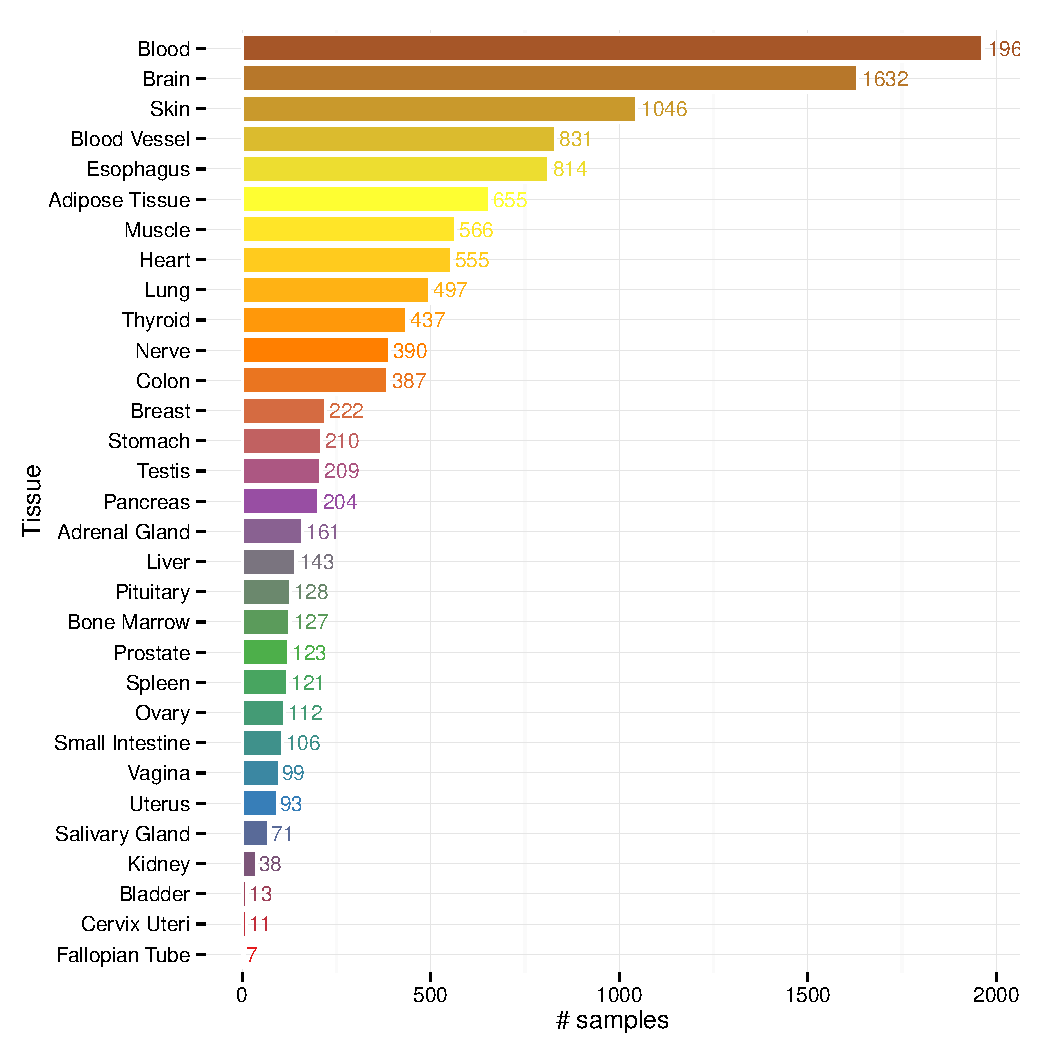
\includegraphics[width=\maxwidth]{figure/samples_per_tissue-1} 
\begin{kframe}\begin{verbatim}
## [1] "Total # of tissues :  30"
## [1] "Total # of samples :  8553"
\end{verbatim}
\end{kframe}
\end{knitrout}

We can see that number of samples per tissue is highly variable. Perhaps this should be considered in the further analysis.

\section{Expression variability per tissue}

Distribution of all the expression values per tissue of 50 randomly sampled transcripts (out of >190 thousand), sampled from the whole GTEx rpkm file. Keep in mind that different tissues have different sample sizes, and thus a different amount of values are plotted on each tissue. \par 
The purpose here is not to compare which tissue has higher or lower expression, or higher or lower variability in expression, but to understand the variability of expression between each tissue, coming from both biological variability and sampling variability. \par
The left-side of the following boxplot contains the distribution of expression values for the sample transcripts using all available samples (e.g. thousands in brain, a handful in Fallopian tube), whereas the right-side boxplot displays the data for the same transcript when only considering 6 (random) samples for each tissue.

\begin{knitrout}
\definecolor{shadecolor}{rgb}{0.969, 0.969, 0.969}\color{fgcolor}\begin{kframe}
\begin{verbatim}
## [1] "ALL SAMPLES: summary(expression_df$value[expression_df$variable == Brain]"
##     Min.  1st Qu.   Median     Mean  3rd Qu.     Max. 
##   0.0000   0.0000   0.0000   3.8380   0.6706 419.8000 
## [1] "ALL SAMPLES: summary(expression_df$value[expression_df$variable == Fallopian Tube]"
##    Min. 1st Qu.  Median    Mean 3rd Qu.    Max.    NA's 
##    0.00    0.00    0.06   13.61    2.49 1035.00   63903 
## [1] "SAMPLED: summary(expression_df$value[expression_df$variable == Brain]"
##    Min. 1st Qu.  Median    Mean 3rd Qu.    Max.    NA's 
##    0.00    0.00    0.00    3.32    0.60   97.94   63903 
## [1] "SAMPLED: summary(expression_df$value[expression_df$variable == Fallopian Tube]"
##    Min. 1st Qu.  Median    Mean 3rd Qu.    Max.    NA's 
##    0.00    0.00    0.06   13.61    2.49 1035.00   63903
\end{verbatim}
\end{kframe}
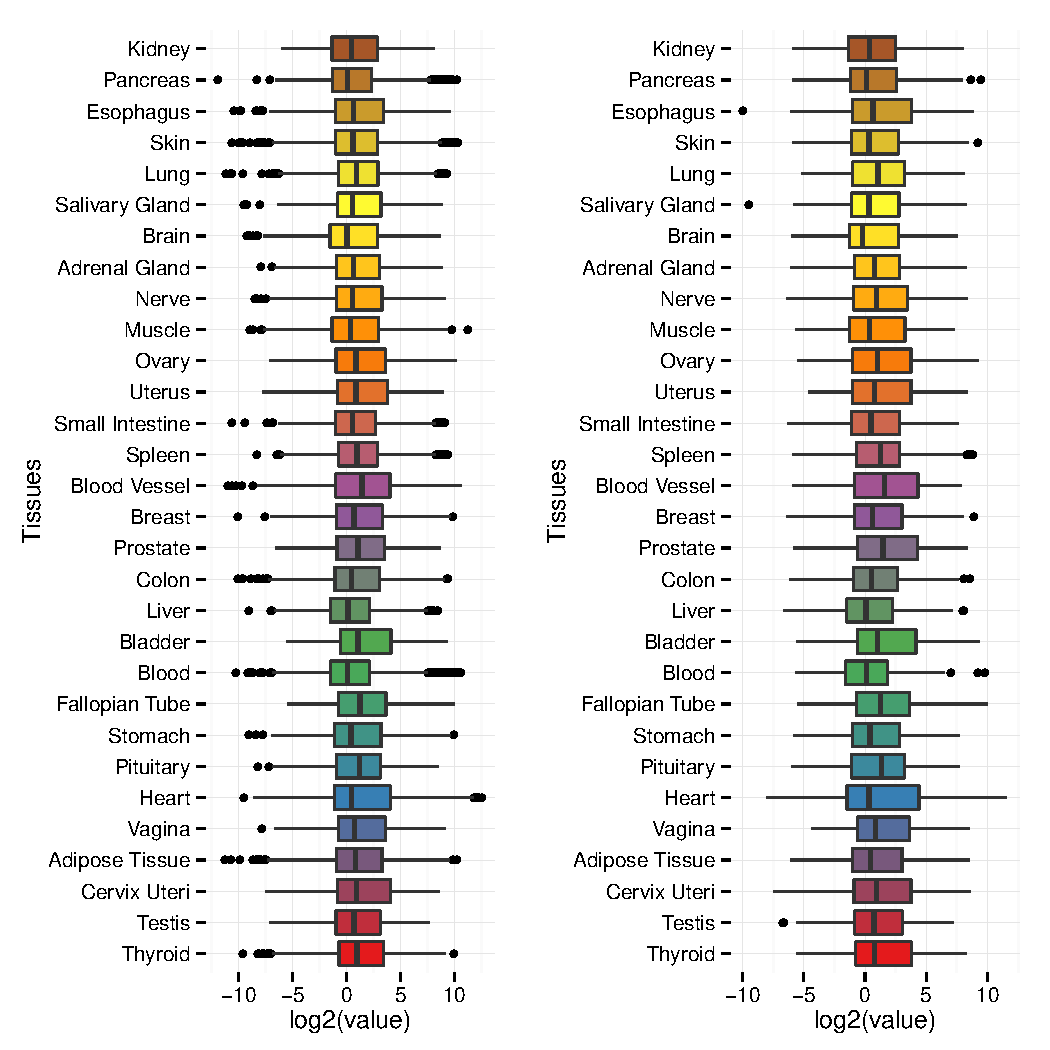
\includegraphics[width=\maxwidth]{figure/expression_per_tissue-1} 

\end{knitrout}

We can see that the number of samples does not drastically change the overal distribution of expression per tissue, only that the number of extreme values (i.e. the black dots) are decresed when reducing number of samples. Thus, as we plan to use some averaging metric between samples of the same tissue for each transcript, we use a different number of samples per tissue, without impairing the credibility or comparibility of the average expression value.

\newpage

\section{Expression distribution per transcript}

Selected 5 tissues with different sample numbers (2 with highest, 1 medium, 2 with lowest sample numbers), randomly selected 12 transcripts and plotted their RPKM value distribution, using all available samples. Note that many transcript have 0 or close to 0 RPKM (*Bug in graphics when all RPKMs are zero) in all addressed tissues. We plan to average the RPKM values of a transcript in a given tissue.

\begin{knitrout}
\definecolor{shadecolor}{rgb}{0.969, 0.969, 0.969}\color{fgcolor}
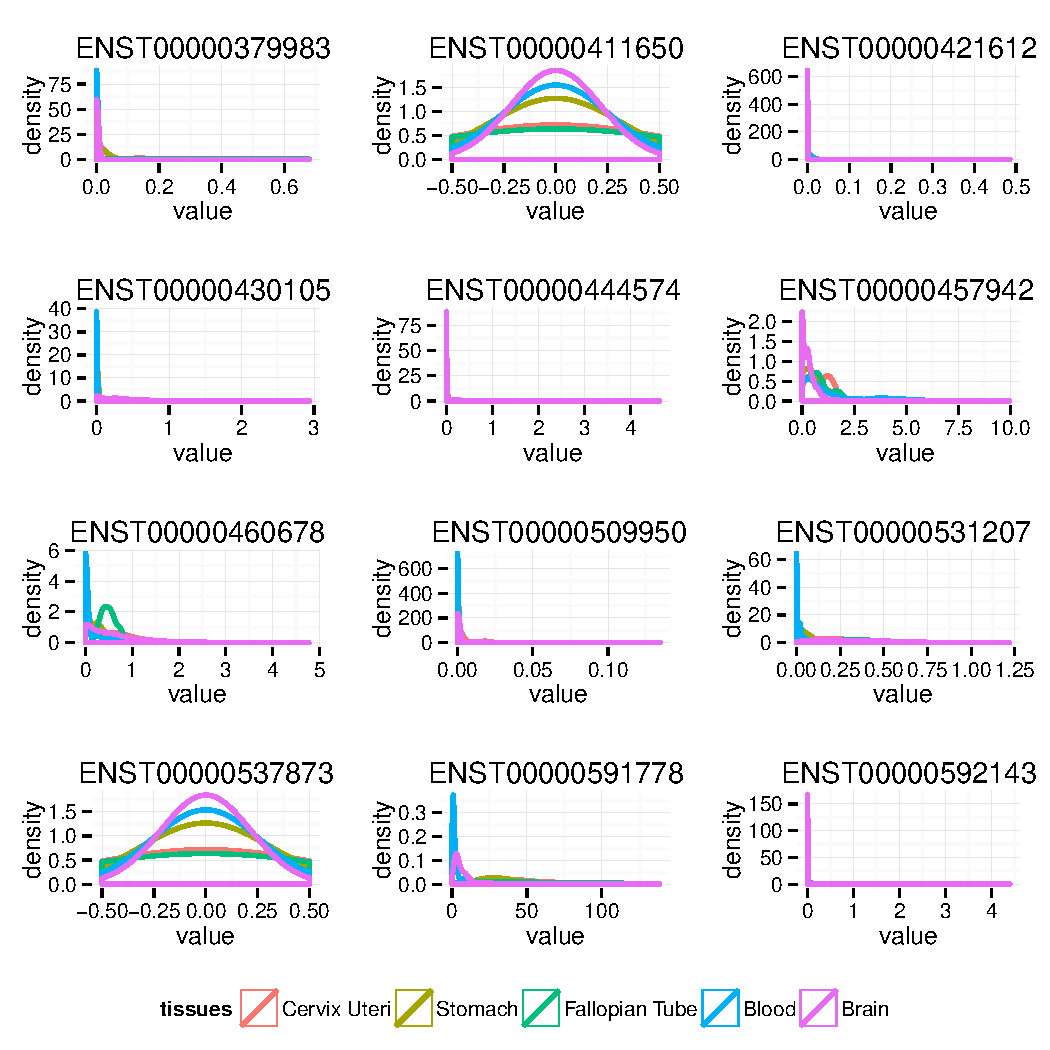
\includegraphics[width=\maxwidth]{figure/density_plot_example_transcripts-1} 

\end{knitrout}

The distributions are highly variable between transcripts. 

\section{Average expression of transcripts per tissue}

To merge sample values within the same tissue and transcript, we can use mean or median. Below are the distributions of averaged RPKM values among all transcripts and all tissues.\par
The blue horizontal lines represent either the mean or the median, the red lines represent the noise cutoff of 0.1 RPKM suggested in the GTEx papers.

\begin{knitrout}
\definecolor{shadecolor}{rgb}{0.969, 0.969, 0.969}\color{fgcolor}\begin{kframe}
\begin{verbatim}
## [1] "summary(expression_df$ExprMean)"
## [1] "summary(expression_df$ExprStd)"
## [1] "summary(expression_df$ExprMedian)"
## [1] "Plots with xlim: 15"
\end{verbatim}
\end{kframe}
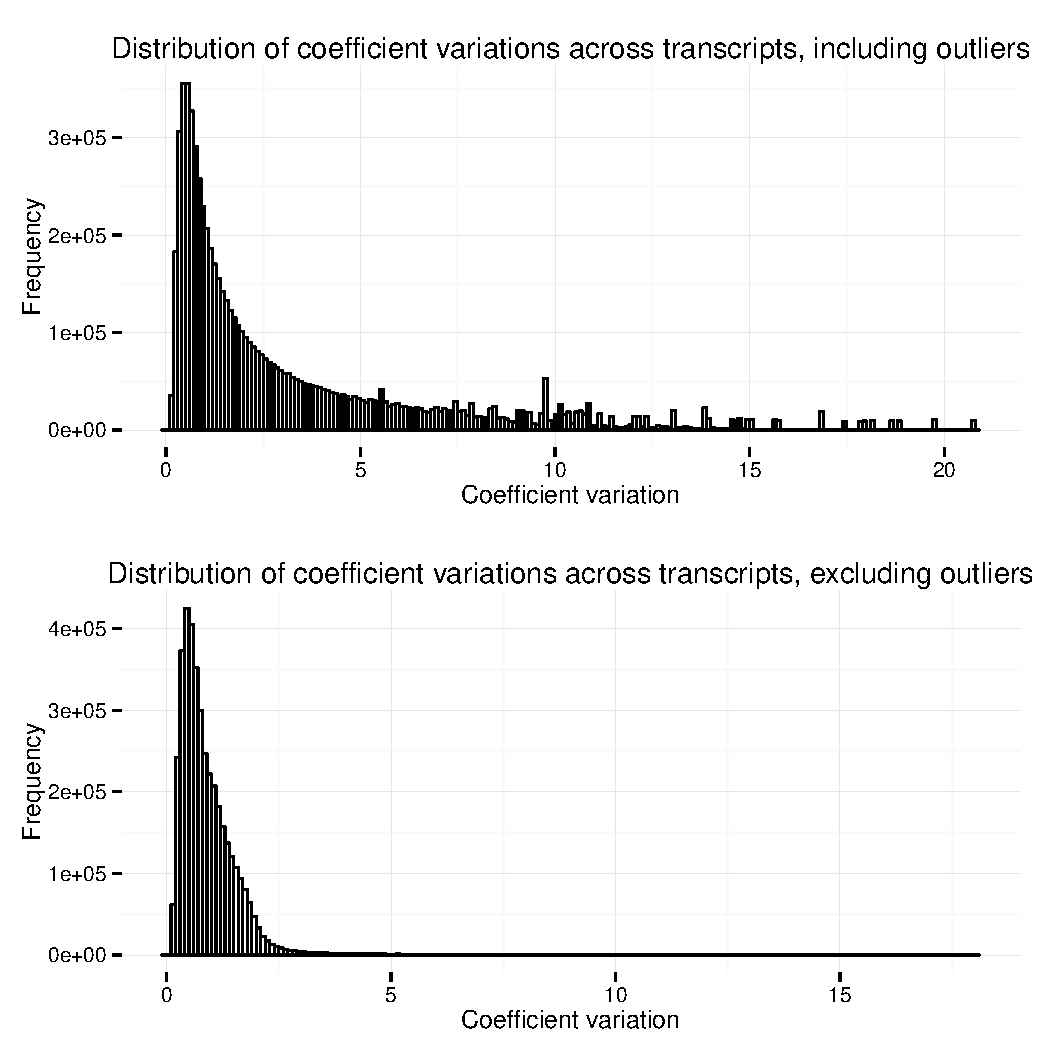
\includegraphics[width=\maxwidth]{figure/transcript_expression_averages-1} 

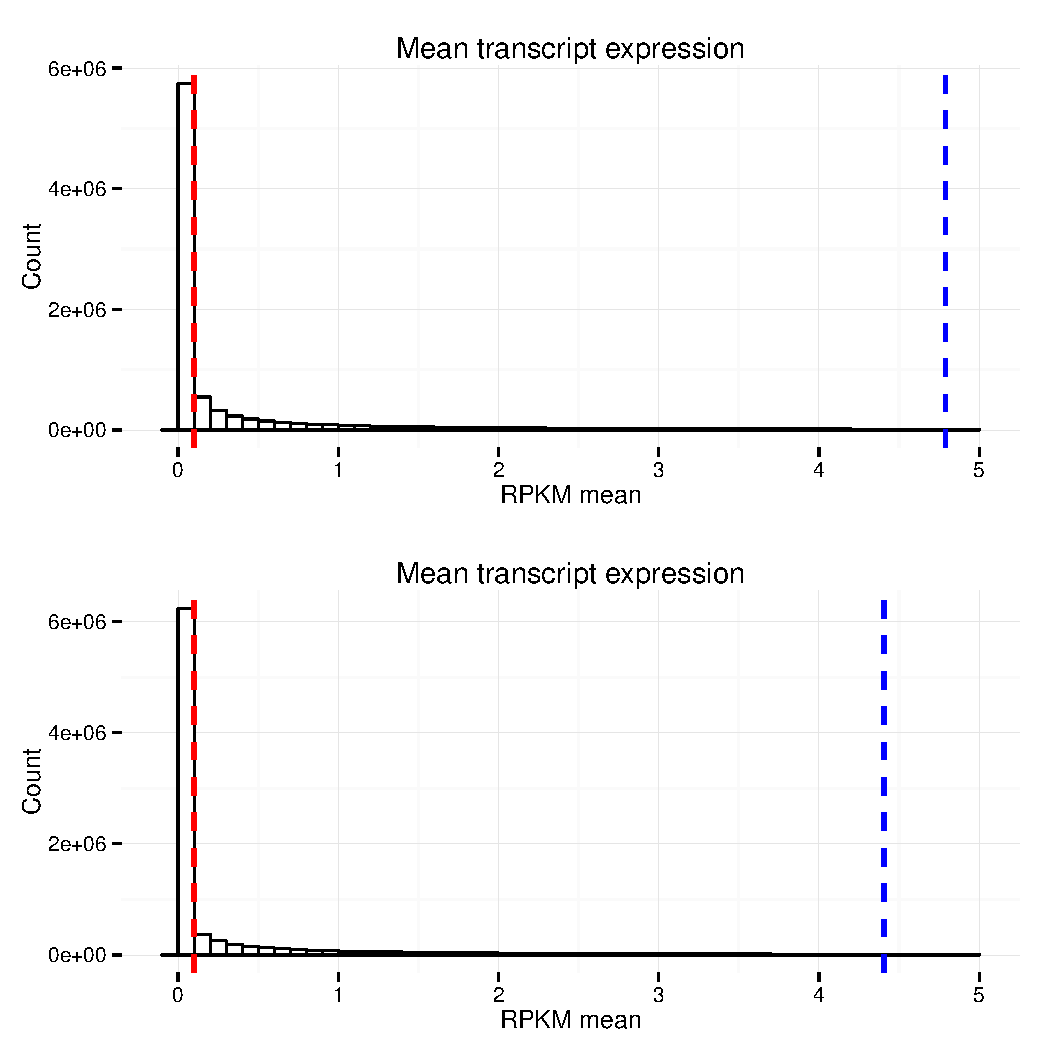
\includegraphics[width=\maxwidth]{figure/transcript_expression_averages-2} 

\end{knitrout}

\section{Conclusion}

We intend to use this expression data not for an expression analysis, but only as a filter layer to ensure lncRNA-protein co-existence in a cell. After setting a rpkm cutoff that distinguishes expression noise from real expression, we will turn our values into binary presence/absence.\par
Because we want to keep the maximum data possible, we do not need to filter out tissues that have low sample numbers, or to normalise data in tissues with a vast number of samples.\\


Parameters for filtering:\\
- minimum rpkm value\\
- interacting pair having to be present in X\% tissues

Need to decide:\\
- what level: tissue or body part?\\

\end{document}

